\documentclass[a4paper]{article}
\usepackage[pdftex]{hyperref}
\usepackage[latin1]{inputenc}
\usepackage[english]{babel}
\usepackage{a4wide}
\usepackage{amsmath}
\usepackage{amssymb}
\usepackage{algorithmic}
\usepackage{algorithm}
\usepackage{ifthen}
\usepackage{listings}
% move the asterisk at the right position
\lstset{basicstyle=\ttfamily,tabsize=4,literate={*}{${}^*{}$}1}
%\lstset{language=C,basicstyle=\ttfamily}
\usepackage{moreverb}
\usepackage{palatino}
\usepackage{multicol}
\usepackage{tabularx}
\usepackage{comment}
\usepackage{verbatim}
\usepackage{color}
\usepackage[utf8]{inputenc}
\usepackage{tabulary}
\usepackage{colortbl}

% Because of an error on line 41 I added this
\usepackage{graphicx}

% Used for drawing DFAs and NFAs
\usepackage{tikz}
\usetikzlibrary{automata, positioning}

%% pdflatex?
\newif\ifpdf
\ifx\pdfoutput\undefined
\pdffalse % we are not running PDFLaTeX
\else
\pdfoutput=1 % we are running PDFLaTeX
\pdftrue
\fi
%\ifpdf
%\usepackage[pdftex]{graphicx}
%\else
%\usepackage{graphicx}
%\fi
\ifpdf
\DeclareGraphicsExtensions{.pdf, .jpg}
\else
\DeclareGraphicsExtensions{.eps, .jpg}
\fi

\parindent=0cm
\parskip=0cm

\setlength{\columnseprule}{0.4pt}
\addtolength{\columnsep}{2pt}

\addtolength{\textheight}{5.5cm}
\addtolength{\topmargin}{-26mm}
\pagestyle{empty}

%%
%% Sheet setup
%% 
\newcommand{\coursename}{Formal Languages and Logic}
\newcommand{\courseno}{CO21-320211}
 
\newcommand{\sheettitle}{Homework}
\newcommand{\mytitle}{}
\newcommand{\mytoday}{\textcolor{blue}{October 11th}, 2018}

% Current Assignment number
\newcounter{assignmentno}
\setcounter{assignmentno}{4}

% Current Problem number, should always start at 1
\newcounter{problemno}
\setcounter{problemno}{1}

%%
%% problem and bonus environment
%%
\newcounter{probcalc}
\newcommand{\exercise}[2]{
  \pagebreak[2]
  \setcounter{probcalc}{#2}
  ~\\
  {\large \textbf{Exercise \textcolor{blue}{\arabic{problemno}}} \hspace{0.2cm}\textit{#1}} \refstepcounter{problemno}\vspace{2pt}\\}

\newcommand{\bonus}[2]{
  \pagebreak[2]
  \setcounter{probcalc}{#2}
  ~\\
  {\large \textbf{Bonus Problem \textcolor{blue}{\arabic{assignmentno}}.\textcolor{blue}{\arabic{problemno}}} \hspace{0.2cm}\textit{#1}} \refstepcounter{problemno}\vspace{2pt}\\}

%% some counters  
\newcommand{\assignment}{\arabic{assignmentno}}

%% solution  
\newcommand{\solution}{\pagebreak[2]{\bf Solution:}\\}

%% Hyperref Setup
\hypersetup{pdftitle={Homework \assignment},
  pdfsubject={\coursename},
  pdfauthor={},
  pdfcreator={},
  pdfkeywords={Formal Languages and Logic},
  %  pdfpagemode={FullScreen},
  %colorlinks=true,
  %bookmarks=true,
  %hyperindex=true,
  bookmarksopen=false,
  bookmarksnumbered=true,
  breaklinks=true,
  %urlcolor=darkblue
  urlbordercolor={0 0 0.7}
}

\begin{document}
\coursename \hfill Course: \courseno\\
Jacobs University Bremen \hfill \mytoday\\
\textcolor{blue}{Dragi Kamov and Dushan Terzikj}\hfill
\vspace*{0.3cm}\\
\begin{center}
{\Large \sheettitle{} \textcolor{blue}{\assignment}\\}
\end{center}

\exercise{}{0}
\solution
\textcolor{blue}{
First we need to check each correlation between each two states and if one of them is an accepting state we are putting a checkmark(blue checkmarks in the table). After that we are checking each pair that has been left unmarked and we are checking when we would be in that state and what would happen if we get a 0 or 1 and if the resulting combination of states is one of the ones checked it is also being checked(red checkmarks). At the end the pairs of states which remain unchecked should be combined together. \\ \\
\begin{tabular}{c|c|c|c|c|c|c}
     & a & b & c & d & e & f \\ \hline
    a & \cellcolor{black} & & & & & \\ \hline
    b & \checkmark & \cellcolor{black} & & & & \\ \hline
    c & \textcolor{red}{\checkmark} & \checkmark & \cellcolor{black} & & & \\ \hline
    d & \checkmark & \textcolor{red}{\checkmark} & \checkmark & \cellcolor{black} & & \\ \hline
    e & \textcolor{red}{\checkmark} & \checkmark & & \checkmark & \cellcolor{black} & \\ \hline
    f & \checkmark & \textcolor{red}{\checkmark} & \checkmark & & \checkmark & \cellcolor{black} \\
\end{tabular} \\ \\
\textcolor{red}{$ (c,a) - \delta(c,0) = e $ \\
\tab $ \delta(a,0) = b $ \\
$ (d,b) - \delta(d,0) = f $ \\
\tab $ \delta(b,0) = a $\\
$ (a,e) - \delta(a,0) = b $ \\
\tab $ \delta(e,0) = e $ \\
$ (f,b) - \delta(f,0) = f $ \\
\tab $ \delta(b,0) = a $} \\
$ (d,f) - \delta(d,0) = f $ \\
\tab $ \delta(f,0) = f $ \\
\tab $ \delta(d,1) = f $ \\
\tab $ \delta(f,1) = f $ \\
$ (c,e) - \delta(c,0) = e $ \\
\tab $ \delta(e,0) = e $ \\
\tab $ \delta(c,1) = f $ \\
\tab $ \delta(e,1) = f $ \\
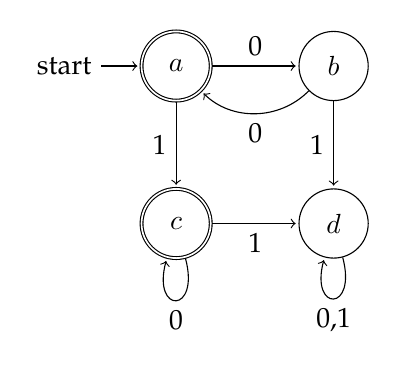
\begin{tikzpicture}[shorten >=1pt,node distance=2cm,on grid,auto] 
   \node[state,initial,accepting] (a)   {$ a $}; 
   \node[state,accepting] (c) [below=of a] {$ c $}; 
   \node[state] (b) [right=of a] {$ b $}; 
   \node[state](d) [right=of c] {$ d $};
    \path[->] 
    (a) edge node {0} (b)
        edge node [swap] {1} (c)
    (b) edge [bend left=45] node [below] {0} (a)
        edge node [swap] {1} (d)
    (c) edge [loop below] node {0} ()
        edge node [swap] {1} (d)
    (d) edge [loop below] node {0,1} ();
\end{tikzpicture}}

\exercise{}{0}
\solution
\textcolor{blue}{
    Let $M=\bigcup\limits_{i=1}^{n} M_{i}$ and let $\Sigma^k=M$. Basically, M is a regular language over $\Sigma$ which accepts words of length $k$ (as denoted in the problem statement). We need to decide whether $L=M$. In order to do that first we need to construct DFAs $A_L$ and $A_M$ for languages L and M respectively. Then we need to minimize $A_L$ and $A_M$ and see whether the two minimized DFAs are identical. 
}

\end{document}
